%\VignetteEngine{knitr::knitr}
%\VignetteIndexEntry{R/Bioconductor package for visualization of phylogenetic networks in a ggplot2 framework.}
\documentclass{article}\usepackage[]{graphicx}\usepackage[usenames,dvipsnames]{color}
% maxwidth is the original width if it is less than linewidth
% otherwise use linewidth (to make sure the graphics do not exceed the margin)
\makeatletter
\def\maxwidth{ %
  \ifdim\Gin@nat@width>\linewidth
    \linewidth
  \else
    \Gin@nat@width
  \fi
}
\makeatother

\definecolor{fgcolor}{rgb}{0.251, 0.251, 0.251}
\newcommand{\hlnum}[1]{\textcolor[rgb]{0.816,0.125,0.439}{#1}}%
\newcommand{\hlstr}[1]{\textcolor[rgb]{0.251,0.627,0.251}{#1}}%
\newcommand{\hlcom}[1]{\textcolor[rgb]{0.502,0.502,0.502}{\textit{#1}}}%
\newcommand{\hlopt}[1]{\textcolor[rgb]{0,0,0}{#1}}%
\newcommand{\hlstd}[1]{\textcolor[rgb]{0.251,0.251,0.251}{#1}}%
\newcommand{\hlkwa}[1]{\textcolor[rgb]{0.125,0.125,0.941}{#1}}%
\newcommand{\hlkwb}[1]{\textcolor[rgb]{0,0,0}{#1}}%
\newcommand{\hlkwc}[1]{\textcolor[rgb]{0.251,0.251,0.251}{#1}}%
\newcommand{\hlkwd}[1]{\textcolor[rgb]{0.878,0.439,0.125}{#1}}%
\let\hlipl\hlkwb

\newenvironment{knitrout}{}{} % an empty environment to be redefined in TeX
\usepackage{alltt}
\usepackage{amsmath}
\usepackage[utf8]{inputenc}
\usepackage[T1]{fontenc}
\usepackage{url}

\RequirePackage[]{/Library/Frameworks/R.framework/Versions/3.6/Resources/library/BiocStyle/resources/tex/Bioconductor}
\AtBeginDocument{\bibliographystyle{/Library/Frameworks/R.framework/Versions/3.6/Resources/library/BiocStyle/resources/tex/unsrturl}}


\IfFileExists{upquote.sty}{\usepackage{upquote}}{}
\begin{document}
%\SweaveOpts{concordance=TRUE}


\bioctitle{The \Biocpkg{ggnetworx} package for visualization of phylogenetic
networks in a ggplot2 framework. }

\author{Klaus Schliep \thanks{\email{klaus.schliep@gmail.com}}\\
University of Massachusetts Boston}

\maketitle

\tableofcontents

\newpage
\section{Introduction}
\Biocpkg{ggnetworx} extends the \Biocpkg{ggtree}\cite{Yu2017} package to allow
visualize several types of phylogentic networks using the \CRANpkg{ggplot2}
\cite{Wickham2016} syntax.
More specific \Biocpkg{ggnetworx} contains function
to plot (unrooted, undirected) splits graphs and (directed, rooted) trees with
reticulations. It offers an alternative to the plot functions already available
in \CRANpkg{ape} and \CRANpkg{phangorn}.

\section{Splits graphs}
Splits graph allow to non-compatible splits definition and are most often
used to visualize Consensus Networks \cite{Holland2004} or Neighbor-Nets
\cite{Bryant2004}. This can be either done using the consensusNet or neighbor-net
function in \CRANpkg{phangorn}\cite{Schliep2011} or by importing nexus files
from SplitsTree \cite{Huson2006}.

We first read the necessary libraries and read in a splits graph
\begin{knitrout}
\definecolor{shadecolor}{rgb}{0.941, 0.941, 0.941}\color{fgcolor}\begin{kframe}
\begin{alltt}
\hlkwd{library}\hlstd{(phangorn)}
\hlkwd{library}\hlstd{(ggnetworx)}
\end{alltt}


{\ttfamily\noindent\itshape\color{messagecolor}{\#\# Loading required package: ggplot2}}\begin{alltt}
\hlstd{fdir} \hlkwb{<-} \hlkwd{system.file}\hlstd{(}\hlstr{"extdata/trees"}\hlstd{,} \hlkwc{package} \hlstd{=} \hlstr{"phangorn"}\hlstd{)}
\hlstd{Nnet} \hlkwb{<-} \hlkwd{read.nexus.networx}\hlstd{(}\hlkwd{file.path}\hlstd{(fdir,}\hlstr{"woodmouse.nxs"}\hlstd{))}
\end{alltt}
\end{kframe}
\end{knitrout}

We can plot a splits graph using:
\begin{knitrout}
\definecolor{shadecolor}{rgb}{0.941, 0.941, 0.941}\color{fgcolor}\begin{kframe}
\begin{alltt}
\hlkwd{ggnetworx}\hlstd{(Nnet)} \hlopt{+} \hlkwd{geom_tiplab2}\hlstd{()}
\end{alltt}
\end{kframe}\begin{adjustwidth}{\fltoffset}{0mm}
\includegraphics[width=\maxwidth]{figure/unnamed-chunk-2-1} \end{adjustwidth}
\end{knitrout}
Nodes can be annotated with $geom_point$.
\begin{knitrout}
\definecolor{shadecolor}{rgb}{0.941, 0.941, 0.941}\color{fgcolor}\begin{kframe}
\begin{alltt}
\hlkwd{ggnetworx}\hlstd{(Nnet)} \hlopt{+} \hlkwd{geom_point}\hlstd{(}\hlkwd{aes}\hlstd{(}\hlkwc{shape}\hlstd{=isTip,} \hlkwc{color}\hlstd{=isTip),} \hlkwc{size}\hlstd{=}\hlnum{3}\hlstd{)}
\end{alltt}
\end{kframe}\begin{adjustwidth}{\fltoffset}{0mm}
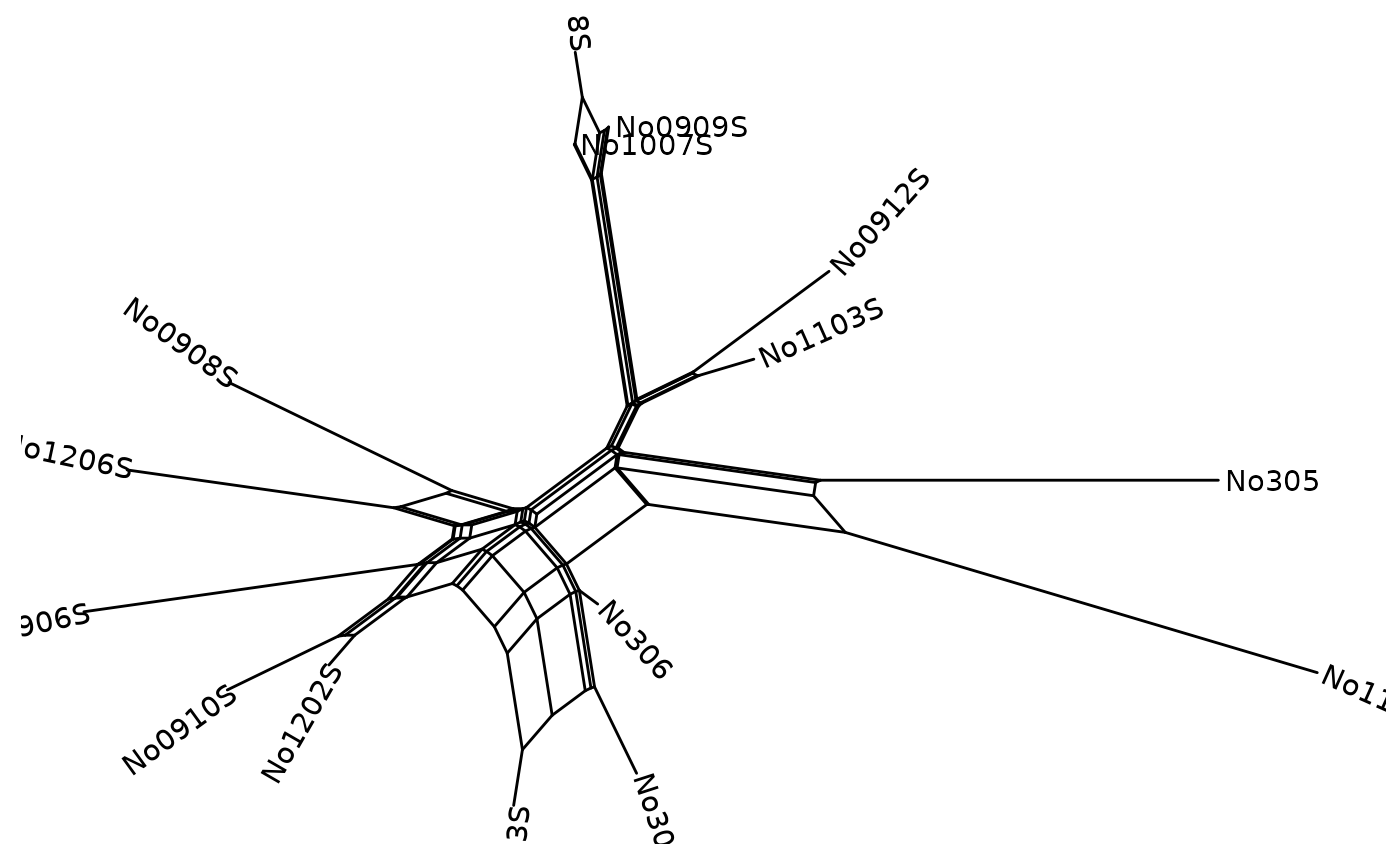
\includegraphics[width=\maxwidth]{figure/unnamed-chunk-3-1} \end{adjustwidth}
\end{knitrout}


\section{Plotting reticulation networks}

The function \Rfunction{ggevonet} plots phylogenetic trees with reticulation.
A recent addition to the \CRANpkg{ape}\cite{Paradis2018}  made it possible
to read in trees in extended newick format \cite{Cardona2008}.

\begin{knitrout}
\definecolor{shadecolor}{rgb}{0.941, 0.941, 0.941}\color{fgcolor}\begin{kframe}
\begin{alltt}
\hlcom{## from Fig. 2 in Cardona et al. 2008:}
\hlstd{z} \hlkwb{<-} \hlkwd{read.evonet}\hlstd{(}\hlkwc{text} \hlstd{=}
         \hlstr{"((1,((2,(3,(4)Y#H1)g)e,(((Y#H1, 5)h,6)f)X#H2)c)a,((X#H2,7)d,8)b)r;"}\hlstd{)}
\hlkwd{ggevonet}\hlstd{(z,} \hlkwd{aes}\hlstd{(}\hlkwc{color}\hlstd{=hybridEdge))} \hlopt{+} \hlkwd{geom_tiplab}\hlstd{()} \hlopt{+} \hlkwd{geom_nodelab}\hlstd{()}
\end{alltt}
\end{kframe}\begin{adjustwidth}{\fltoffset}{0mm}
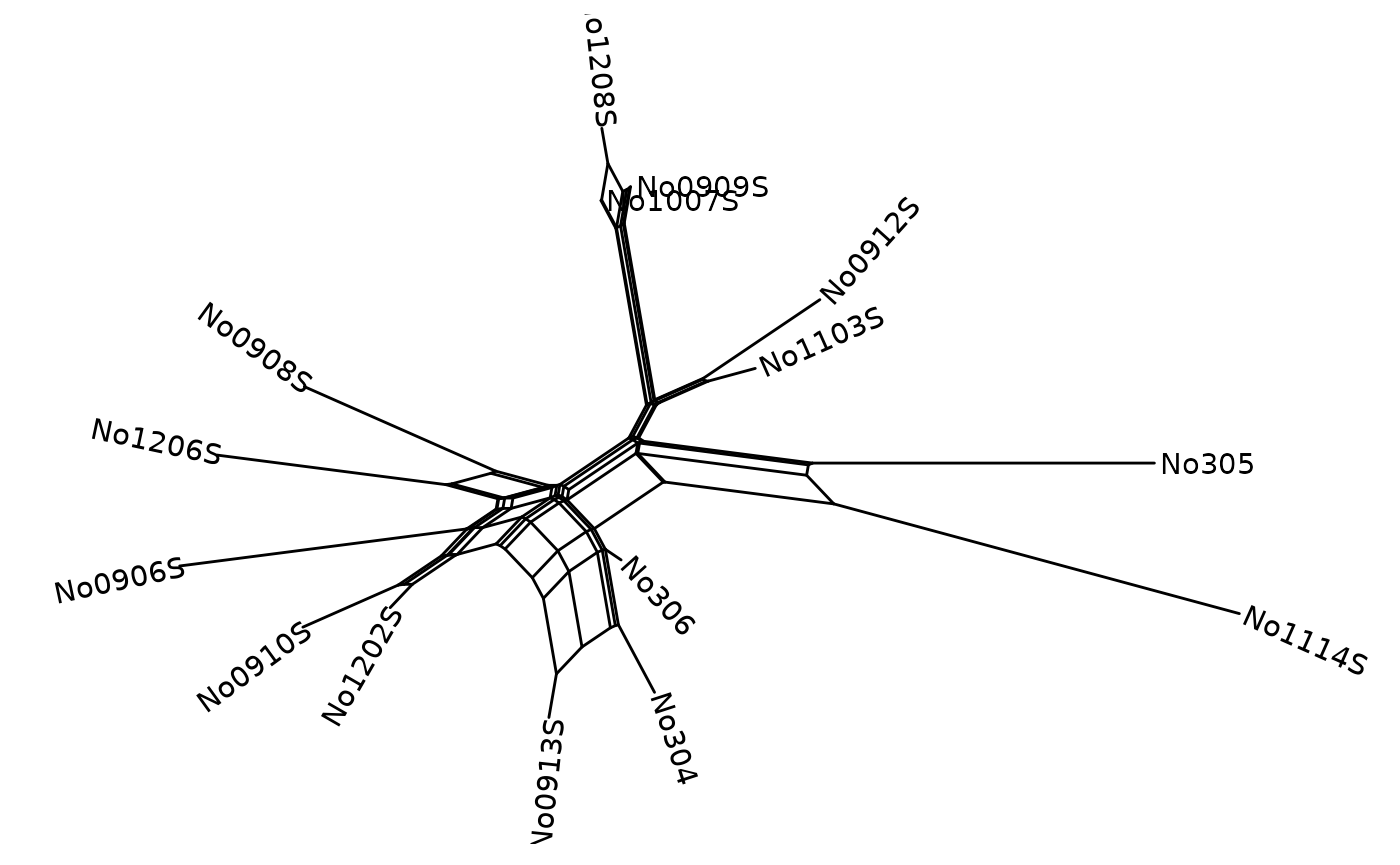
\includegraphics[width=\maxwidth]{figure/unnamed-chunk-4-1} \end{adjustwidth}\begin{kframe}\begin{alltt}
\hlkwd{ggevonet}\hlstd{(z,} \hlkwd{aes}\hlstd{(}\hlkwc{color}\hlstd{=hybridEdge),} \hlstr{"slanted"}\hlstd{)} \hlopt{+} \hlkwd{geom_tiplab}\hlstd{()} \hlopt{+} \hlkwd{geom_nodelab}\hlstd{()}
\end{alltt}
\end{kframe}\begin{adjustwidth}{\fltoffset}{0mm}
\includegraphics[width=\maxwidth]{figure/unnamed-chunk-4-2} \end{adjustwidth}
\end{knitrout}

\section{Summary}

The splits graph should take most of the functions which go with unrooted
trees in ggtree. The reticulation graphs are phylogram or slanted.
Not all options may not work as intended yet.

\url{https://bioconductor.org/packages/devel/bioc/vignettes/ggtree/inst/doc/treeVisualization.html}



\nocite{Schliep2011}
\nocite{Schliep2017}
\nocite{Paradis2004}
% \nocite{Paradis2018}
\nocite{Holland2004}
\nocite{Yu2017}
\nocite{Bryant2004}
\nocite{Huson2006}
\nocite{Cardona2008}
\nocite{Wickham2016}


\newpage
\bibliography{ggnetworx}

\newpage
\appendix
\section{Session info}
\begin{knitrout}
\definecolor{shadecolor}{rgb}{0.941, 0.941, 0.941}\color{fgcolor}\begin{kframe}
\begin{alltt}
\hlkwd{sessionInfo}\hlstd{()}
\end{alltt}
\begin{verbatim}
## R version 3.6.1 (2019-07-05)
## Platform: x86_64-apple-darwin15.6.0 (64-bit)
## Running under: macOS Mojave 10.14.6
## 
## Matrix products: default
## BLAS:   /Library/Frameworks/R.framework/Versions/3.6/Resources/lib/libRblas.0.dylib
## LAPACK: /Library/Frameworks/R.framework/Versions/3.6/Resources/lib/libRlapack.dylib
## 
## locale:
## [1] en_US.UTF-8/en_US.UTF-8/en_US.UTF-8/C/en_US.UTF-8/en_US.UTF-8
## 
## attached base packages:
## [1] stats     graphics  grDevices utils     datasets  methods   base     
## 
## other attached packages:
## [1] ggnetworx_0.1.0 ggplot2_3.2.1   phangorn_2.5.5  ape_5.3        
## [5] ggtree_2.1.1    knitr_1.25     
## 
## loaded via a namespace (and not attached):
##  [1] Rcpp_1.0.2         highr_0.8          pillar_1.4.2      
##  [4] compiler_3.6.1     BiocManager_1.30.9 tools_3.6.1       
##  [7] zeallot_0.1.0      digest_0.6.22      jsonlite_1.6      
## [10] tidytree_0.2.9     lifecycle_0.1.0    evaluate_0.14     
## [13] tibble_2.1.3       nlme_3.1-141       gtable_0.3.0      
## [16] lattice_0.20-38    pkgconfig_2.0.3    rlang_0.4.1       
## [19] igraph_1.2.4.1     fastmatch_1.1-0    Matrix_1.2-17     
## [22] rvcheck_0.1.6      yaml_2.2.0         parallel_3.6.1    
## [25] xfun_0.10          treeio_1.11.0      withr_2.1.2       
## [28] dplyr_0.8.3        stringr_1.4.0      vctrs_0.2.0       
## [31] grid_3.6.1         tidyselect_0.2.5   glue_1.3.1        
## [34] R6_2.4.0           rmarkdown_1.16     purrr_0.3.3       
## [37] tidyr_1.0.0        magrittr_1.5       backports_1.1.5   
## [40] scales_1.0.0       htmltools_0.4.0    assertthat_0.2.1  
## [43] BiocStyle_2.14.0   colorspace_1.4-1   labeling_0.3      
## [46] quadprog_1.5-7     stringi_1.4.3      lazyeval_0.2.2    
## [49] munsell_0.5.0      crayon_1.3.4
\end{verbatim}
\end{kframe}
\end{knitrout}

\end{document}
